\documentclass[12pt]{extreport}
\usepackage[vmargin=1in]{geometry}   
\usepackage{graphicx}
\usepackage{url}
\usepackage[utf8]{inputenc}
\usepackage{tikz}
\usepackage{gantt}
\usepackage{rotating}

\usepackage{fontspec,xltxtra,xunicode}
\defaultfontfeatures{Mapping=tex-text}

\setromanfont[Mapping=tex-text]{Times}
\begin{document}

%\renewcommand{\chaptername}{}
\title{Project Proposal\\ \huge{Estimating the Real World Usage of Image Steganography }}
\author{Ritesh Kumar Sinha\\ 1006510\\MSc(IT) 2010-2011}

\date{\today}

\maketitle
\begin{abstract}
Image steganography provides an alternative means of communication between parties wishing to share secrets in an environment where the use of cryptography alone may not be feasible.  This proposal outlines the design and implementation of an experiment  that would help estimate the use of image steganography as a means of covert communication on the Internet by analysing publicly available images available on the World Wide Web.      
\end{abstract}
\pagenumbering{roman}
\tableofcontents




\pagenumbering{arabic}

\chapter{Introduction}
\label{ch:intro}
This chapter provides an overview of steganography and a background of the problem domain. The problem that this project intends to study is described in more detail in Section \ref{sec:probstatement}. We discuss the origins of steganography, historical implementations and modern techniques that enable data hiding in plain sight. 
\section{Background}
The use of steganographic techniques to hide messages in everyday objects is thought to have existed for thousands of years. The Greek historian Herodotus tells the story of Demeratus who wanted to inform his friends in Greece of an impending Persian invasion  \cite{kahn1996history}. Demeratus is said to have concealed the message in writing tablets that, to the casual observer, appeared to be blank tablets covered with wax. The hidden message was written on the wooden tablet and was discovered by the recipients after melting the wax covering it.   

Contemporary methods of digital steganography, on the other hand, utilise redundant data found in digital files to hide messages in plain sight  \cite{hinson2009introduction}.  This is made possible by the fact that digital media contains a large amount of redundant information. Subtle changes made to this redundant data are not readily detectable by visual inspection as shown in Fig \ref{fig:stegexample}.  If the message to be hidden is relatively short in comparison to the size of the file, this encoding ensures that the original and modified files appear exactly the same to the casual observer.
\begin{figure}[h!]
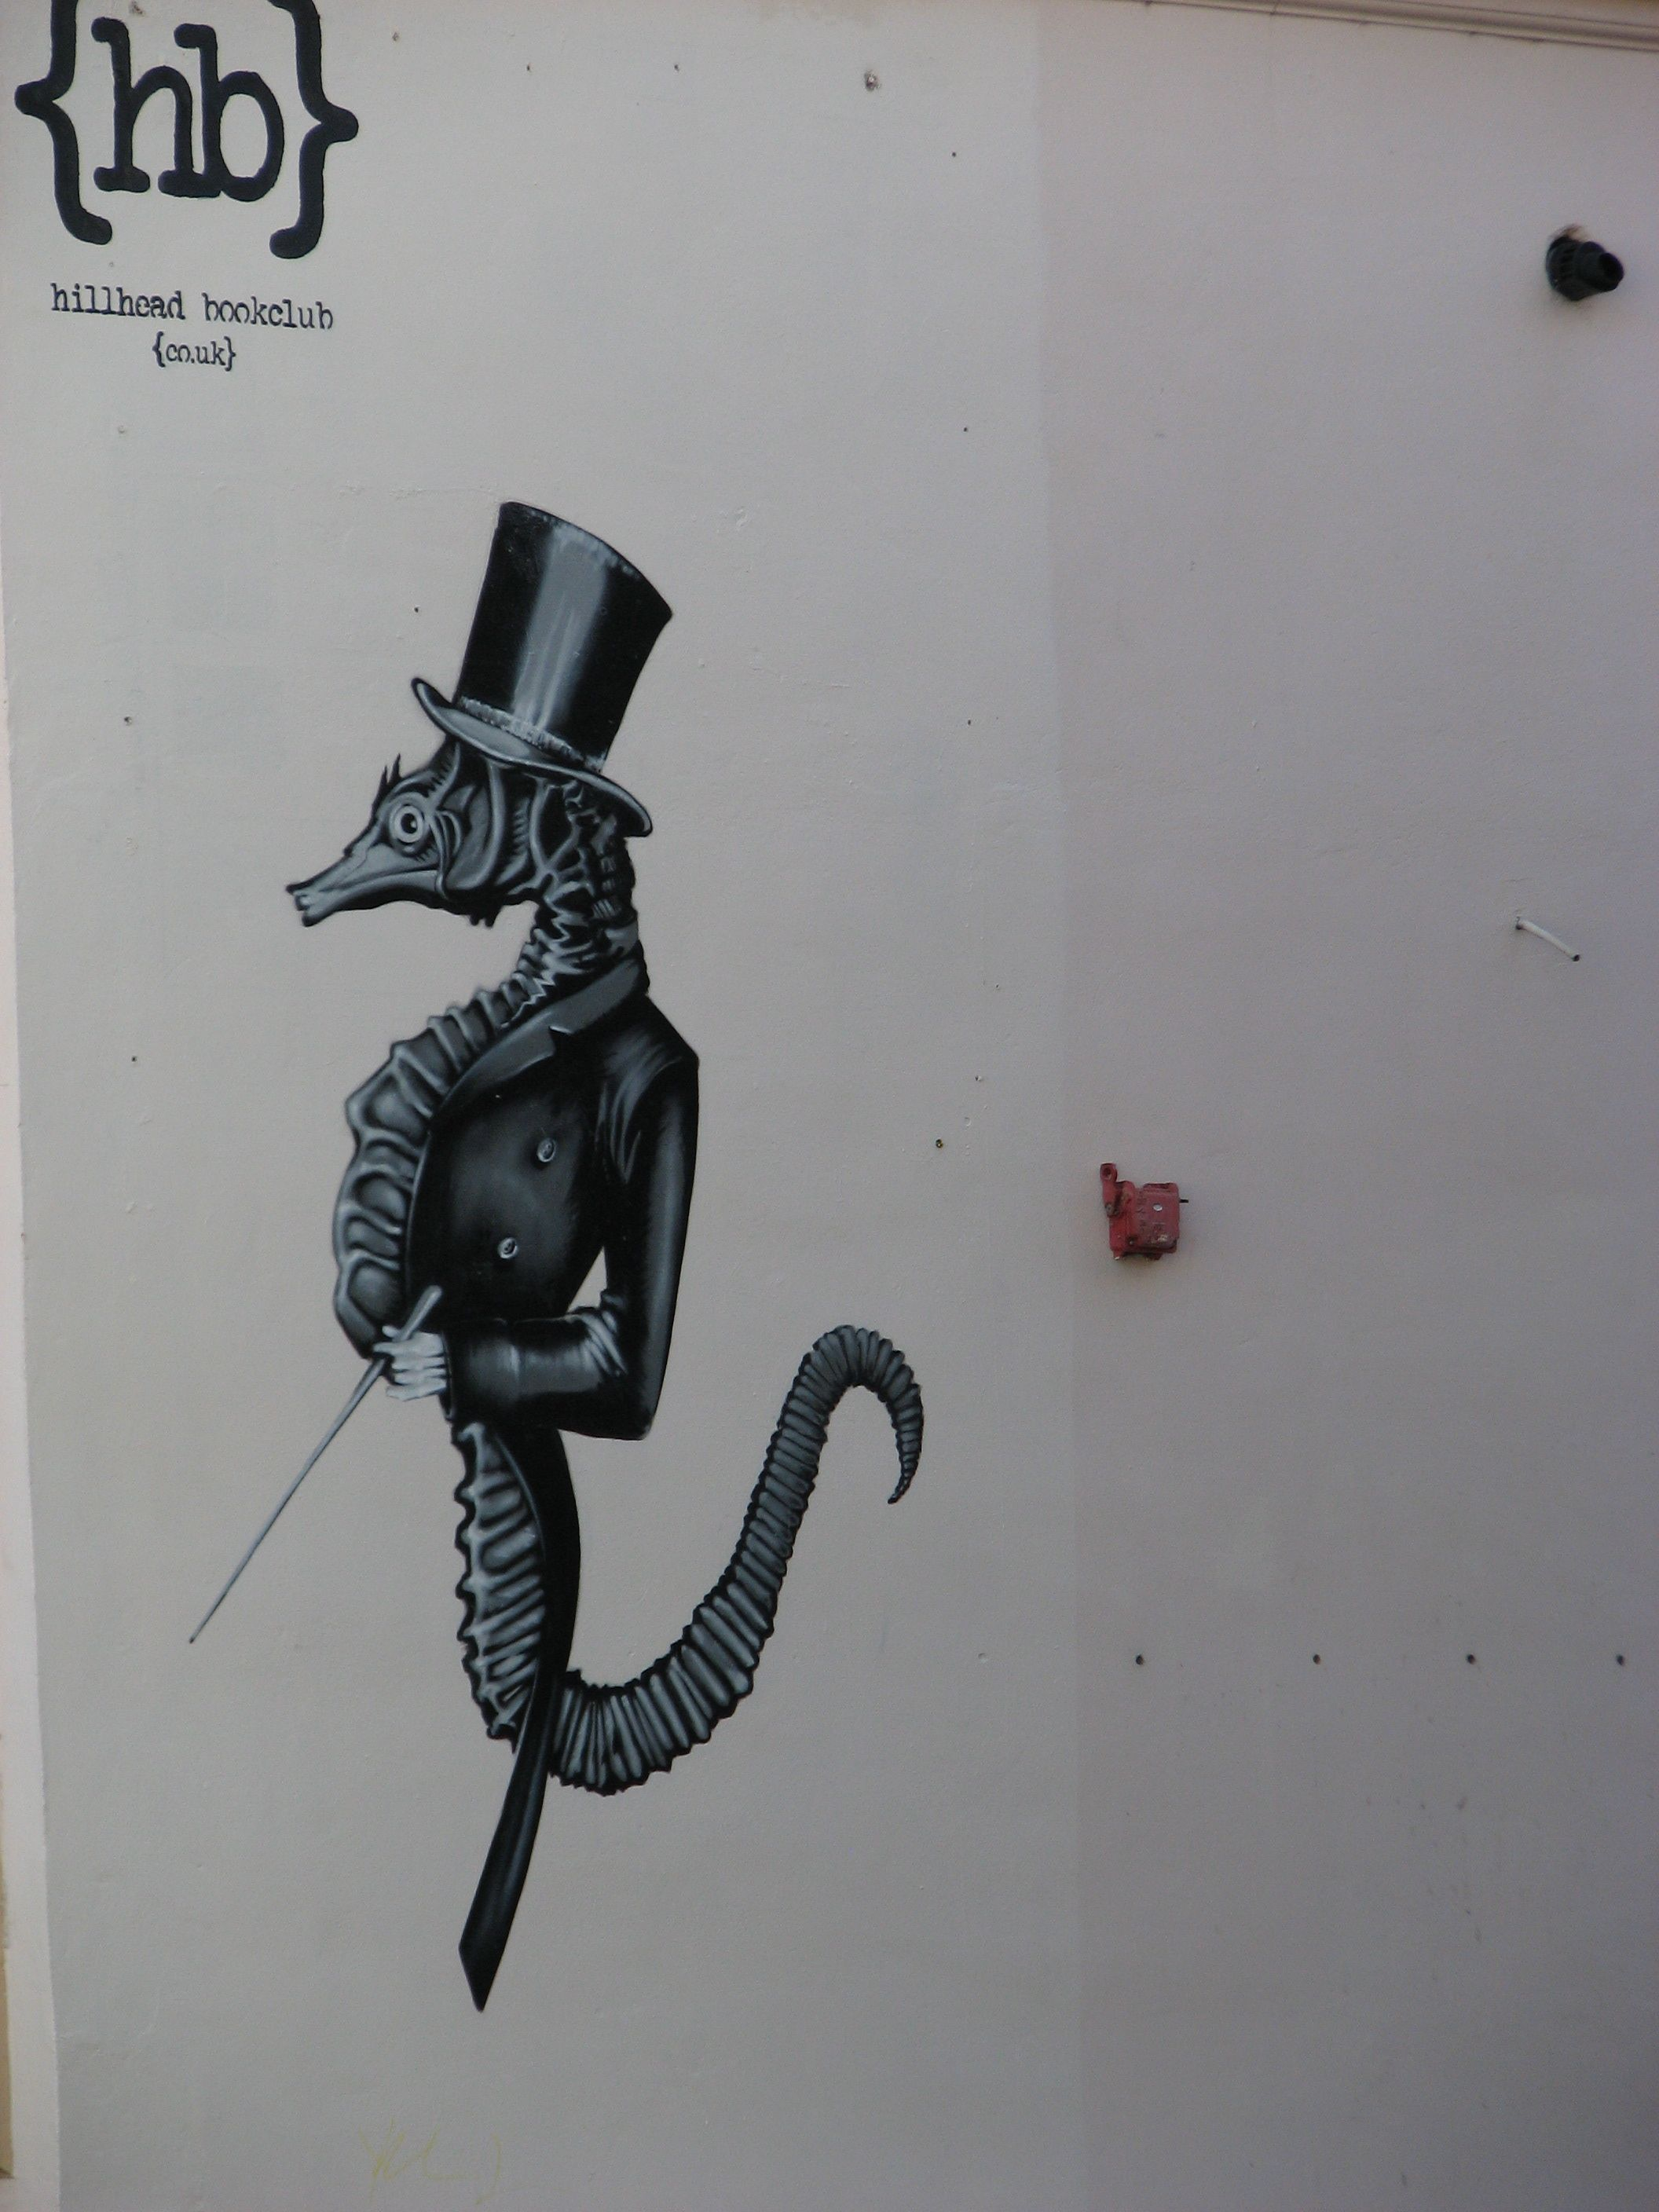
\includegraphics[scale=0.10]{hb1}
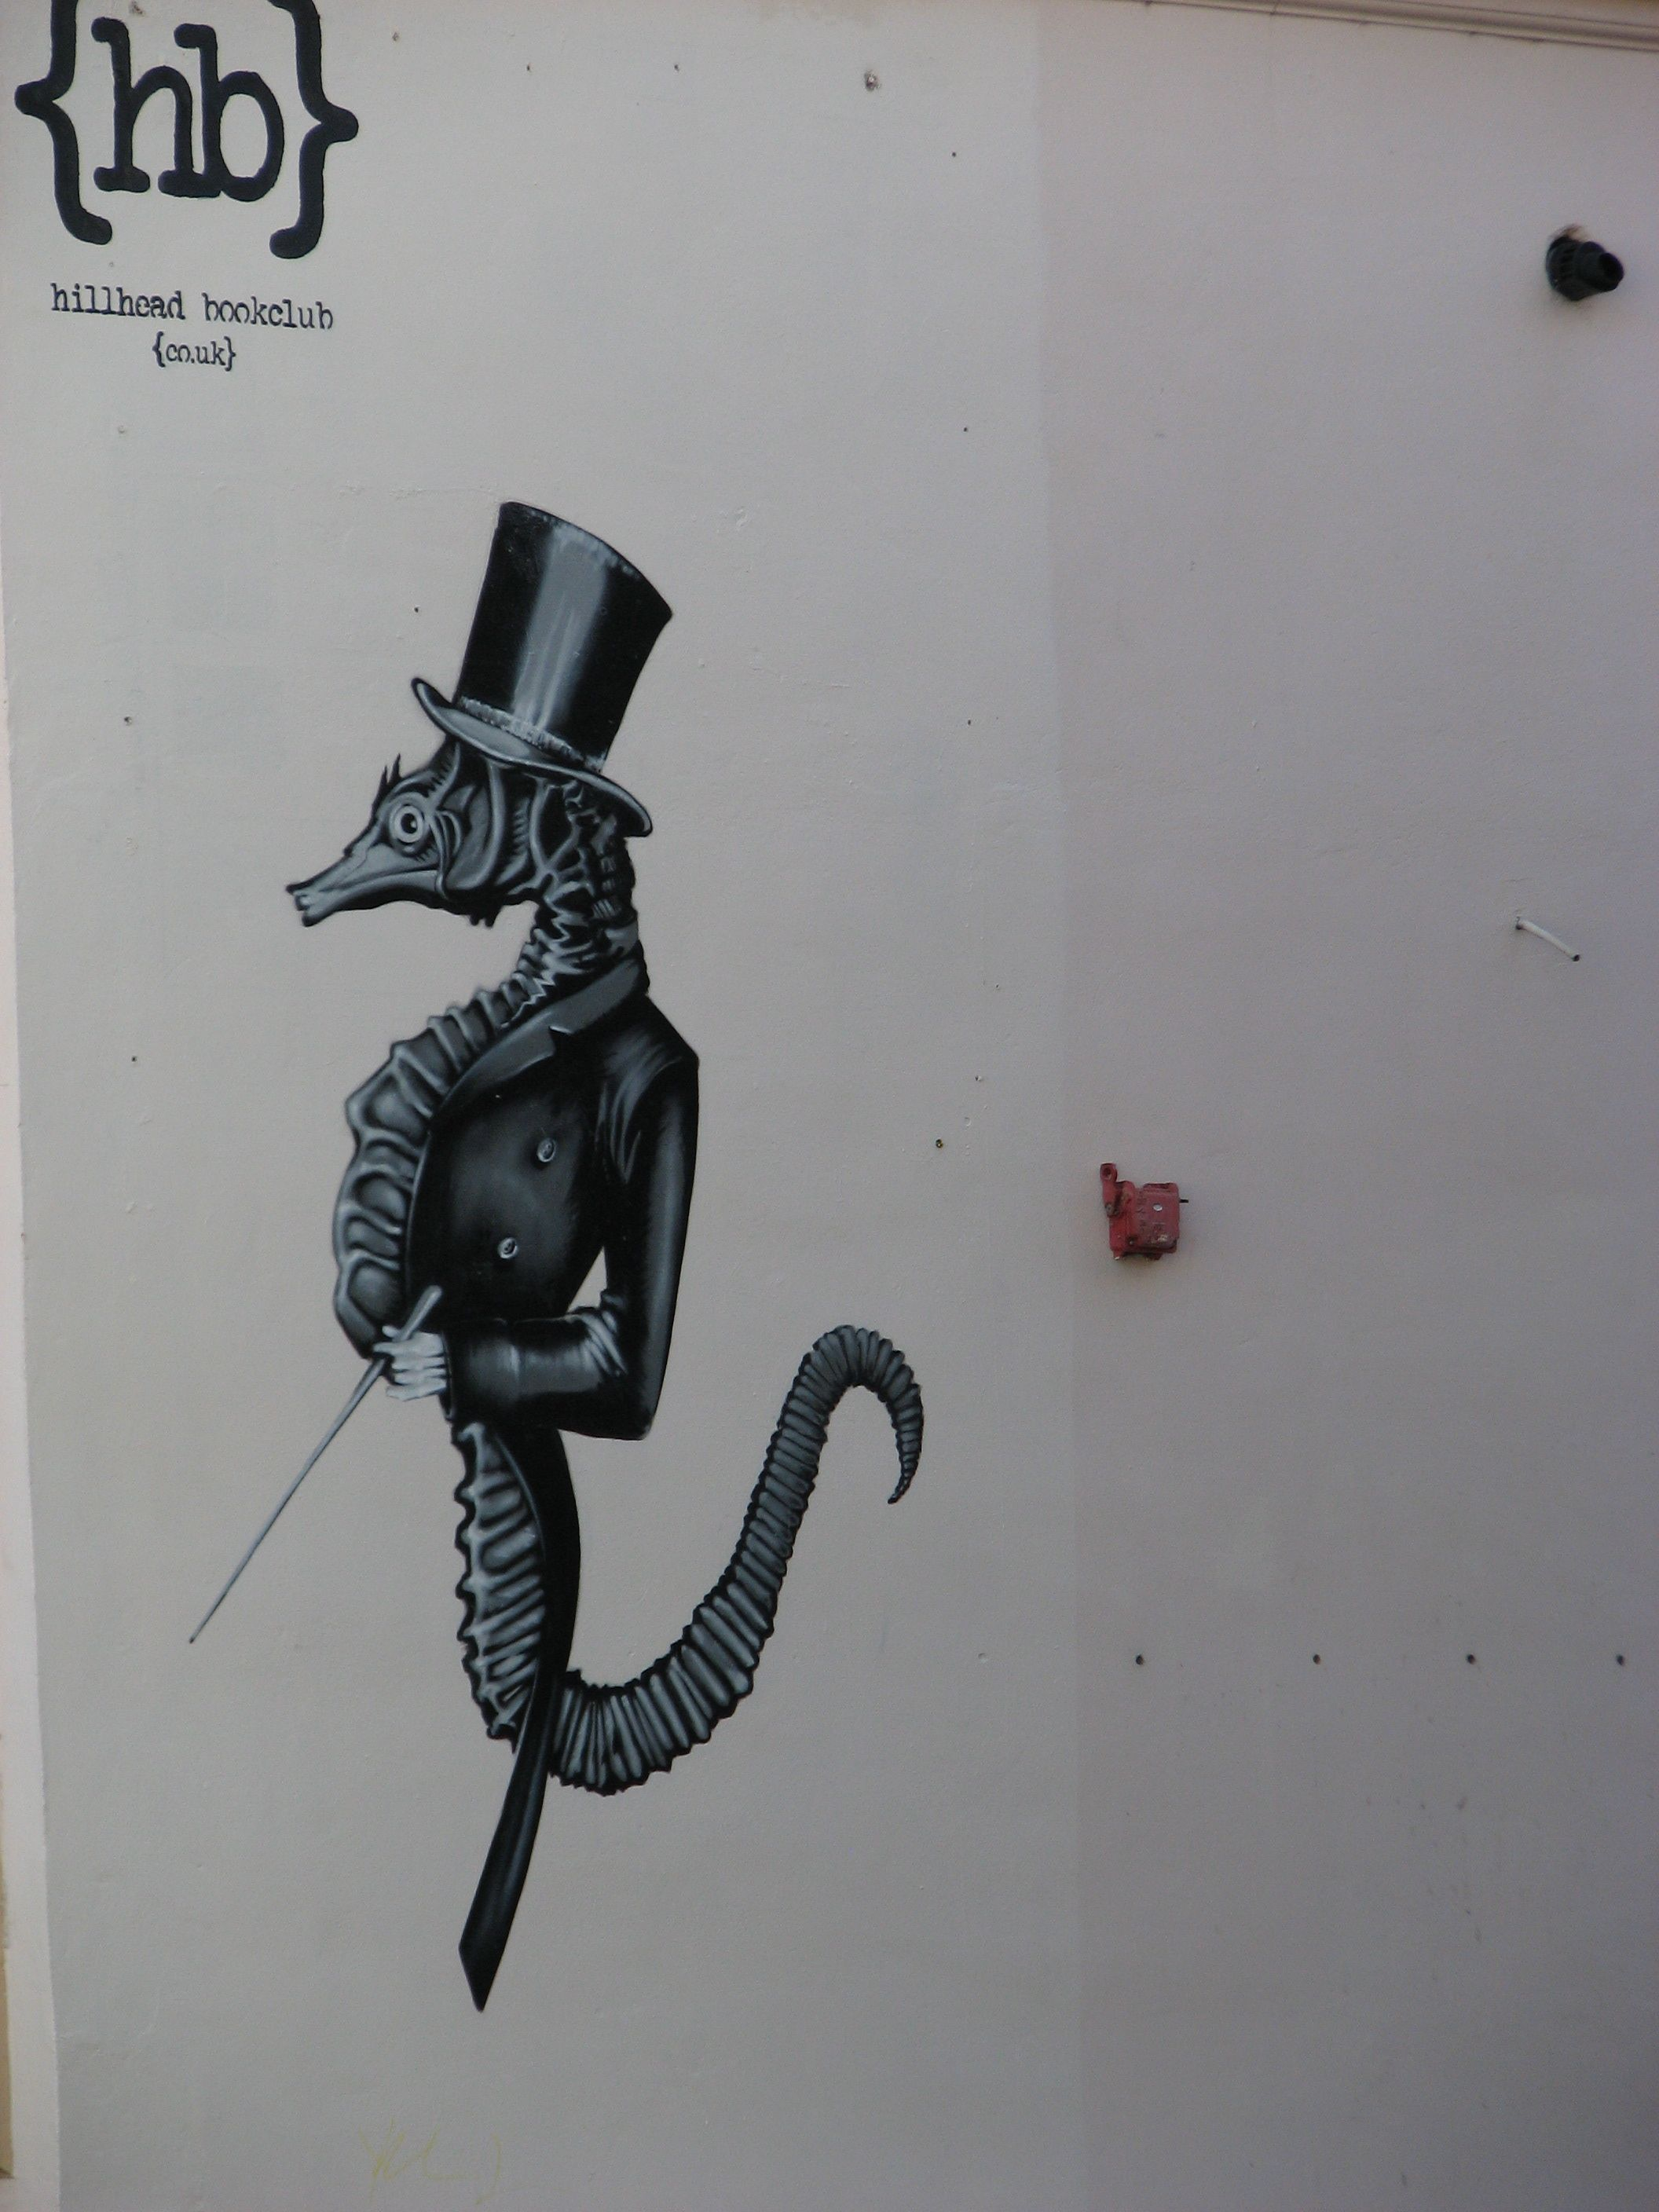
\includegraphics[scale=0.10]{hb1}
\caption{\emph{The images above show that there are no obvious differences between an unaltered image and the same image with data embedded in it using open source steganographic software called Stepic \cite{stepnic}. The image on the right contains the following text embedded using steganography : ``Thoughts, words, and deeds, the statute blames with reason;  But surely dreams were ne'er indicted treason \cite{burns}"}}
\label{fig:stegexample}
\end{figure} All digital mediums \cite{pan2007intelligent} can be used to hide data using this method, including audio \cite{crawford2010supraliminal} and text \cite{shirali2006new}. Image steganography is thought to be the most widely used form. This is perhaps due to the large number of freely available tools that allow one to embed data in images. A na\^{\i}ve steganographic implementation would not attempt to encrypt the data before embedding it in the image. Most popular steganographic tools, however, allow the user to encrypt the data with a password before embedding the secret text. The hidden message can then be recovered by the recipient with a suitable decoding tool and the correct password or decryption key. This makes image steganography a viable medium for covert communication.  
Another common use of steganography is for the purposes of copyright enforcement  \cite{kundur2002digital}. Using digital watermarks that contain copyright information,  it is possible to uniquely identify an image even after it has  been modified. These ``marks'' can be read by specialised software which can determine the original source of the image.
\par The use of steganography as a covert communication channel on the internet has always been a contentious topic and a source for much speculation. Analysis of a terrorist user manual, the Technical Mujahid \cite{alfajr}, by the United States Central Intelligence Agency (CIA) mentioned chapters in that outline various concealment techniques utilising image based steganography. The manual describes the use of steganography as an additional layer of security over encrypted data. It's however, difficult to ascertain whether these techniques are in use in the real world. An argument for the limited use of steganography would be that steganography is an approach that relies on security through obscurity. Security through obscurity implies the use of a secret, but insecure, method of protecting a resource. An example of this would be hiding one's room keys under the doormat in the hope that a thief would never find it there. In 2000, Provos and Honeyman \cite{provos2001detecting}  carried out an analysis of images available on eBay for steganographic content.  They argue that either there isn't  significant use of steganography on the internet or that the steganographic techniques used are undetectable by the methods used by them. They also concede that it might be possible that encryption might have been used on the data embedded in the images and that they were unable to decrypt it. Their analysis is based on a fairly large (2 million) image dataset acquired from eBay.   More recent news reports  \cite{spies2010} suggest that members of a Russian spy ring arrested in the United States in 2010 used steganography to communicate with each other. Reports speculate that these individuals posted images with steganographic content on public image hosting sites with sensitive data embedded in them. The news reports, however, did not provide any technical details regarding the steganography methods used. This provides an opportunity to revisit the seminal work conducted by Provos \emph{et al} to try and establish real world usage of steganography.

It would be trivial to prove the \emph{existence} of steganography if one were provided the unaltered host image along with the image carrying the steganographic payload. By calculating the binary difference of the steganographic image from the unaltered image, one could easily discover the payload embedded in the image. However, this is an unrealistic expectation in the real world as the steganographic host medium will be less likely to be found along with the altered copy. Hence it is necessary to explore other means for the steganalysis of images that do not require the original host image for comparison.


\section{Problem Statement}
\label{sec:probstatement}
It would be trivial to prove the \emph{existence} of steganography if one were provided the unaltered host image along with the image carrying the steganographic payload. By calculating the binary difference of the steganographic image from the unaltered image, one could easily discover the payload embedded in the image. However, this is an unrealistic expectation in the real world as the steganographic host medium will be less likely to be found along with the altered copy. Hence it is necessary to explore other means for the steganalysis of images that do not require the original host image for comparison.

In this proposal, a number of methods for detecting steganographic content in publicly accessible image files are explored. It is proposed that the images required for this analysis will be limited to a set of random public websites especially those that encourage posting of user generated content. The analysis of images for steganographic content will be referred to as steganalysis. The identification of steganographic content is of primary concern, attempts to recover the encoded message will be made only if their is sufficient time remaining. An experimental setup is proposed that would allow for the collection and analysis of images for steganographic analysis. The results from this research will be used to estimate real world usage of steganography. 
\section{Structure of Proposal}
\label{sec:structure}
In Section \ref{sec:probstatement} the problem that the project aims to address is stated. Chapter \ref{ch:bgsurvey} contains the background survey that was carried out to better understand the problem domain and previous work carried out in this area. Section \ref{sec:theory} discusses important papers describing theoretical attacks on steganographic systems. Section \ref{sec:tools} explores a number of tools that are available today for creating steganographic images. Sections \ref{sec:steganalysistools} \& \ref{sec:practicalattacks} discuss available steganalysis tools and practical attacks on steganographic systems. This brings us to the motivation behind carrying out further research in this area which is described in Section \ref{sec:motivation}. In Chapter \ref{ch:papproach} an approach towards the design and implementation of a an experimental setup that would aid acquire images from the internet and subsequently analyse them for steganographic content is described. Chapter \ref{ch:workplan} contains the task breakdown and the proposed work plan. 

\chapter{Background Work}
\label{ch:bgsurvey}
In this section, prior work in the field of image steganalysis is explored. This chapter is divided into two sections; the first section addresses literature that was found to be relevant to this study and the second section evaluates a number of software tools that implement image steganography.  In the literature survey, both theoretical and practical attacks on steganography are examined. The theoretical works  form the basis of practical steganalytic implementations that follow. 
The following sections describe previous publications of work in the field of theoretical and practical attacks against steganography. While the field of steganography is not limited to images, the scope of this project is limited to the analysis of image based steganographic systems. 
\section{Approaches to Image Steganography}
\label{sec:overview}
Before moving on to the analysis of steganographic images, it is important to establish context by understanding the various approaches to steganography. A large amount of literature exists on different ways to encode data in digital content. For the purpose of this project, only image based steganography is of interest. In particular we are interested in implementations that allow data hiding in image types that are likely to be uploaded to the Internet. This includes JPEG, GIF and PNG images.
\par There are a number of tools available that provide steganography features; either as data hiding tools or for digital watermarking purposes. Our interest is limited to steganographic tools that are explicitly designed for data hiding purposes but it may be worthwhile to explore non standard uses of popular digital watermarking tools enabling covert information hiding for communication. 
\par Overall, most popular tools implement either or all of the following types of steganographic algorithms along with an optional layer of encryption.
\begin{itemize}
\item Least Significant Byte image encoding:  LSB encoding is perhaps the most simple form of steganography. It is implemented by overwriting the least significant bit of each pixel in an image with part of the secret message. One of the key disadvantages of LSB encoding is that data is not preserved if the image is resized or edited. This form of steganography is also relatively easy to identify merely by visual inspection if the host (unaltered) version of an image is available.
\item Frequency Domain Encoding: This is a slightly more sophisticated steganographic technique and is implemented in a number of tools like JSteg \cite{jsteg}. A digital image consists of a number of pixels that represent colour values. Furthermore, each colour value has a specific frequency in an image. The frequency distribution can be transformed into a ring structure by using a function called the 2D Fast Fourier Transform. The resultant pattern resembles a ring with the lower frequencies represented at the centre and the higher frequencies towards the edges. By converting a digital image into its constituent  frequency distribution and subsequently using a 2D FFT function, it is possible to utilise the mid-range frequency to store data. Both LSB encoding and Frequency Domain Encoding require images that are approximately 3 times larger than the message to be encoded. Frequency Domain Encoding provides better protection against the discovery of the secret message and is marginally affected by file compression. 
\item BPCS encoding : Bit-Plane Complexity Segmentation Based Embedding is a relatively new and potentially more effective way of data hiding.  A digital image can be segmented into a number of bitplanes of increasing complexity \cite{kawaguchi1998concept}. This segmentation divides the image into planes in such a way that each plane contributes some amount of detail to an image. The higher order planes contain the most detail and represent the features available in the image. The lower order planes contribute very little and appear as noise when viewed on their own.  For an image of size $n$ it is possible to use as much as $\frac{n}{2}$ of the image for hiding data provided that the image is sufficiently complex. For simpler images, any alteration to lower order bit planes that constitute the image would be readily evident.

\end{itemize}
\section{Theoretical Work in Steganalysis}
\label{sec:theory}
Pfitzmann and Westfield \cite{westfeld2000attacks} describe two methods for analysing images for steganographic content. The first method is the use of visual techniques to identify whether an image could contain steganographic content. Based on the presumed  steganography tool used, they attempt to filter all parts of image presumed to contain the secret message. 
After this, it is possible to test if the image could contain steganographic content by observing the filtered image.  
\par The second method utilises the $\chi^{2}$ statistical test to determine if the image contains steganographic content. In this method,  the theoretical expected frequency distribution of pixels in an image is compared with the actual frequency distribution of the pixels in the steganographic image. A deviation between these values indicates the presence of a steganographic message. This is possible as the tools used for creating the steganographic image incorrectly assume that the Least Significant Bits are random and can be overwritten to hide message.
\par Building on the works of Pfitzmann et al  \cite{westfeld2000attacks}, Fridrich and Goljan \cite{fridrich2002practical} present a collection of qualitative methods for practical steganalysis. The authors extend the statistical analysis described by both Pfitzmann and Provos to include the spatial arrangement of pixels in a steganographic image referred to as ``Dual Statistical attacks''. 
\par The JPEG compatibility attack described by Goljan et al relies on finding non compatible JPEG artefacts in images. The image to be analysed is divided into  8x8 pixel blocks and the algorithm attempts to locate blocks that would not ordinarily be produced by the JPEG compression algorithm.
\par A universal, ``meta'' steganalysis approach from Farid  \cite{farid2002detecting} is also described by the author, which attempts to detect the type of steganography used rather than being a targeted approach towards a specific steganographic algorithm.  This approach utilises higher order statistical modelling that provides a generic approach to detect the presence of steganographic content in images. Farid's experimental setup consists of three types of support vector machines (SVMs). A support vector machine is a data classifier with a very high degree of accuracy \cite{noble2006support}. The kernel parameters for the support vector machine were tuned as to provide a very low (1.0\%) false positive rate. They were then trained with a library of GIF, JPEG and TIFF images. The trained SVMs were used to classify a large number of mixed (steganographic and non steganographic) images. It was discovered that with a low false positive rate, a non-linear SVM was able to accurately classify 90.2\% of steganographic images of size $160\times160$ pixels correctly with a false negative rate of 9.8\%.

\section{Survey of Image Steganography Tools}
\label{sec:tools}
In this section an overview of popular steganographic tools is presented. It was found that while a number of tools are available for steganography, many of them share similar algorithms to encode data in digital files.  The tools are evaluated on the basis of their availability, the operating system platforms they support and the algorithm used by them. The design of the user interface or additional features provided by the tools are not of any importance for the purpose of this study as it is assumed that users of the software tools are already familiar with it.
\subsection{EzStego}
EzStego \cite{ezstego} is a free steganographic tool created by Romana Machado  implemented in Java and is available for the most common operating systems (Linux,Windows, MacOS). The software appears to be no longer maintained but copies of it are mirrored in other locations of the web. The steganograms produced by EzStego have been extensively studied by a number of authors  \cite{westfeld2000attacks, farid2002detecting}. It is most susceptible to the visual attack as it relies of Least Significant Bit encoding (LSB) to hide data in a GIF file. 
\subsection{S-Tools}
S-Tools \cite{stools} are a collection of steganographic tools that allow for data hiding in a number of digital file formats. Supported formats include WAV, GIF and BMP files. It is not possible to use a JPEG file as a medium for steganographic data using this software.  S-Tools also allows the user to choose between DES, Triple DES, IDEA and MDC encryption algorithms. In order to recover data from S-Tools created steganograms,  the user is required to know the passphrase that was used as the key to encrypt the data and the encryption algorithm used.  S-Tools is available for Windows and UNIX like operating systems.
\subsection{JSteg} 
JSteg \cite{jsteg} is a steganographic tool that allows a user to embed messages in JPEG files, the message size is limited to roughly 12\% of the image size. It has been extensively studied by a number of authors including Westfeld and Goljan. The image medium used is JPEG, which is a lossy image compression algorithm. Owing to this images containing data encoded with JSteg are immune to traditional visual attacks unlike EzStego, which requires an uncompressed Bitmap image as the medium. Due to the use of JPEG as an the medium, it is not possible to reliably isolate data that is encoded in the least significant bit field and prove the existence of steganography. Steganograms produced by JSteg are, however, still vulnerable to statistical attacks. JSteg is written in C and is available for Windows and UNIX like operating systems.
\subsection{JPHide and Seek}
JPHide and Seek \cite{jphide} was written by Alan Latham and it is exclusively designed to hide data in JPEG images. It's primary design goal is providing plausible deniability \emph{i.e.} it should be difficult or impossible to prove that a particular image contains steganographic data. This goal is acheived if the message length is less than 15\% of the size of the image and the image contains significant detail (\emph{e.g.} a picture of a forest with a river). Separate versions for Windows and Linux are available.
 \subsection{F5}
 The F5 algorithm \cite{westfeld2001f5} was created by Westfeld to provide a steganographic solution that was resilient to both visual and statistical attacks. This is made possible by the design of the F5 algorithm that uses matrix encoding for data and uses permutation techniques to distribute the data throughout the steganographic medium. Unlike LSB based steganography software like JSteg and S-Tools, F5 encodes data by manipulating the DCT coefficients in a JPEG image. 
 \subsection{StegMark}
 StegMark \cite{stegmark} is a commercial software product developed by DataMark Technologies. It is not strictly designed for steganographic communication; instead this software implements digital watermarking using steganography. Digital watermarking can be used to enforce digital content ownership and prevent plagiarism of images or other digital media. It can, however, be used to communicate covertly as it provides an SDK for creating steganography tools. StegMark is available for Windows as a C++ SDK.
 \subsection{Stepic \& ESFS}
 Stepic \cite{stepnic} is a relatively new steganography tool written by Lenny Domnitser in Python. The steganography implementation appears to be pedagogical as it only provides data hiding by using LSB encoding. Another project, the Encrypted Steganographic Filesystem (ESFS) \cite{esfs}, has adapted Stepic to provide a File System in User Space (FUSE) based filesystem for Linux. StegFS also provides an additional security by encrypting the data using AES with a 256 bit key. It is a proof of concept implementation and the author claims that the performance is relatively poor. Stepic is available as open source software for both Windows and UNIX like operating systems while ESFS requires Linux and Python with the cryptographic toolkit (pycrypto) installed.
 \subsection{Digital Picture Envelope}
 Digital Picture Envelope is the result of research \cite{kawaguchi1998concept} in the area of Bit Plane Complexity Steganography(BPCS). This method of steganography is radically different from the other implementations that rely on LSB encoding to hide data. The Digital Picture Envelope converts the host image into a number of bit planes, each plane constitutes part of the image. The most complex planes can be used as information carriers as changes to it cannot be perceived by the human eye.  An added advantage is that unlike other steganographic mechanisms, BPCS \emph{alters} the actual image instead of appending to it thereby ensuring that the steganogram is the same size as the original image. Additionally, up to 50\% of the image can be used to store the data. Digital Picture Envelope is available in binary format for Windows systems only. 
 
\section{Evaluation of Image Steganalysis Tools}
\label{sec:steganalysistools}
In this section we discuss a number of tools that provide steganalysis features. We discussed a number of theoretical attacks on steganographic systems in the previous section. However, there are relatively few tools that implement all steganalysis attacks. For the purpose of our project it is necessary to identify a set of tools that will provide a universal system for steganalysis \emph{i.e.} the tools should be able to prove the existence of steganography in a given image. It would be ideal to be able to identify the steganographic algorithm used but this may not be possible in all cases. Some of the tools that implement steganalysis are:
\begin{itemize}
\item Outguess : Outguess \cite{outguess} ships as a package that provides steganography tools as well steganalysis tools. It implements custom detection routines for popular steganography algorithms like JSteg, F5 and JPHide. It also provides the command line tools stegdetect and stegbreak, the former implements steganography detection while the latter provides a tool that attempts to extract data from a steganogram using brute force and dictionary attack methods. It is available as open source software with source and binaries for all platforms. 
\item Gargoyle : Gargoyle \cite{gargoyle} is a commercial malware removal product that ships with a proprietary database of hashsets. These hashsets provide a method of identifying steganographic content by checking for ``signatures'' left by steganographic software. The software package is available for Windows and is designed for forensic investigators.
\item EnCase : Another commercial software product \cite{encase} that provides various  computer forensic features. It has features that allow for steganographic detection. Encase runs on Windows and employes signature based detection to check for the presence of steganography.
\item AccessData Forensic Toolkit :  This commercial tool allows for the identification of steganography based on proprietary hashsets \cite{ftk}. Like Gargoyle and Encase, it can only identify the presence of steganography in files by means of hash analysis. It is limited to identify a finite number of specific steganography algorithms. 
 
\end{itemize}
The availability of free image steganalysis tools is limited as compared to the numerous options available for image steganography. A few steganography suites, like Outguess \cite{outguess} provide a combined steganography/steganalysis software suite. Commercially available tools like Encase, provide steganalysis as part of a digital forensics toolkit.  
\section{Practical Attacks on Steganographic Systems}
\label{sec:practicalattacks}
An exhaustive study carried out in 2001 by Provos and Honeyman \cite{provos2001detecting} analysed over 2 million images publicly available from eBay auctions using a similar method. Images that were classified as being suspicious were subjected to a dictionary attack in order to attempt recovery of the message.
 \par Their results did not find any significant use of steganography in images that were posted as part of the auctions. However they do not discount the possibility that the images they analysed were using steganographic techniques that were not not detectable by the methods employed by them.
\par For the few thousand images that were discovered to have been marked as suspicious by their setup, it was not possible to recover any of the messages embedded in them.  They speculate that it could have been due the use of a strong password to encrypt the message stored in the images.
\section{Motivation for Further Research}
\label{sec:motivation}
While the work of Provos and Honeyman appear to have little success in finding steganographic images on the internet based on a sample of about 3 million images  \cite{provos2001detecting} gathered from eBay, their study was done at a time when social media networks and personal web pages were not as popular as they are today. With the proliferation of user created content on the internet and recent debates regarding the real world usage of steganography, it is important to establish whether these claims hold any merit. The development of a steganography detection platform would, apart from determining real world usage of steganography, provide an experimental framework for repeatable research in this area in the future.\\
In the following chapter, a proposed approach to create an experimental setup to address the problem described in Section \ref{sec:probstatement} is described. 
\chapter{Proposed Approach}
\label{ch:papproach}
The design of the experiment is implemented as four components that would provide the necessary features to address the problem statement. Each of these components must work independently of each other in order to allow for separation of concerns, as well as allowing for the possibility of running them on separate machines. 
\begin{enumerate}
\item \emph{Web Crawler Module} :
Web crawling refers to the process of methodically browsing the Internet as a human being would; it starts from a specified URL and discovers subsequent URLs to browse to from the pages it has already crawled. The ``crawler'' or ``spider'' is the software component that performs this process, which, after starting from the initial URL, discovers subsequent URLs and visits them in turn. 
The crawler attempts to download images in every page it finds and saves them in a location that the decision component can find and send to the analysis component for further analysis.  However, the crawler is restricted to a depth of 3 links per page to ensure that it does not attempt to traverse a site indefinitely. It is hypothesised that if there are images with steganographic content in the site, it should be available in plain view and not hidden within the site. There is a bandwidth penalty associated with crawling to a large depth and it could also cause the experiment to exceed the time-frame provided.  It is proposed to use Scrapy \cite{scrapy}, an open source web crawling framework to implement this module.
 
\item \emph{Decision Module} : 
As many pages on the Internet are mirrored are other locations either by accident or intentionally, it is required that duplicate images (images that have already been sent for analysis) are not sent for analysis a second time. The decision module produces a cryptographic hash of the image downloaded by the crawler and looks up the hash in the database. Each image stored in the database has its own cryptographic hash as its primary key. This is a slight modification of the approach adopted by Provos et al, which directly pipes all images downloaded to the steganalysis component. It is assumed that our approach will ensure optimum resource utilisation without compromising on the quality of the data analysed. This is possible due to the fact that it is highly improbable for two images to have the same cryptographic hash  \cite{wang2005collision}.

\item \emph{Steganalysis Module} :
This component would provide the implemented steganalysis features. This module may have a number of steganalysis sub modules that implement different forms of steganography detection. The aim is to provide a uniform interface to different methods of analysis. The steganalysis module would connect to the database that contains images that have been marked for steganalysis and attempt to analyse them. If any of the modules flag the image as being suspicious the image is marked for further review.

\item \emph{Reporting module} :
This module would provide reporting facilities that would help track the progress of the experiment. In particular it would allow the experimenter to view statistics regarding the number of images analysed, the number of websites crawled etc. This could be implemented as a text based interface to a database that stores these statistics or as a web front-end to a database table that contains statistics from the running experiment.
 
\end{enumerate}
\section{Experimental Setup}
\label{sec:expsetup}
Fig \ref{fig:setup} illustrates the proposed experimental setup designed to address the problem referred to in Section \ref{sec:probstatement}. 
The experimental setup will be composed of a crawler module, a decision module, a steganalysis module and a database.The crawler module will be fed with a series of start URLs to begin crawling. 
\par Based on the seed URLs subsequent URLs will be discovered by parsing the contents of the starting URLs. The crawler will attempt to locate image files at these URLs and forward them to the decision module. 
\par The decision module decides if the image has already been encountered by calculating the cryptographic hash of the image (SHA1) and looking it up in the database. If the image exists, the image is discarded from the temporary store. If not, the image is stored in the database.
\par The steganalysis module obtains images from the database and attempts to test them for steganographic content using interfaces to tools or custom statistical tests. If the image is found to contain steganographic content, it is marked for further research in the database. If not, the image is marked as analysed.
\par The images (both analysed and marked for further research) are preserved until all results have been consolidated.The system is proposed to be implemented in Python as there are a number of readily available libraries which could be re-used to build the experimental setup.  

\begin{center}
\begin{figure}
\includegraphics[angle=90, width=0.9\textwidth]{arch.png}
\caption{Experimental Setup}
\label{fig:setup}
\end{figure}
\end{center}
 

\chapter{Work Plan}
\label{ch:workplan}
This section outlines the proposed work plan for the project.  Fig \ref{fig:gantt} shows the Gantt chart for the project. The task breakdown structure along with the estimated time required is as follows :
\begin{itemize}
  \item Experiment with web crawler to identify an efficient implementation for the project : 0.5 Week
  \item Implementation of decision module to interface with crawler and database : 1 Week
  \item Implementation of statistical steganalysis module : 1.5 Weeks
  \item Testing of experimental framework : 2 Weeks
  \item Experiment running time : 4 Weeks
  \item Analysis of results : 1 week
  \item Finalising the dissertation : 2 weeks 
\end{itemize}  
  The dissertation will be worked on from the start to the finish of the project. If the experiment yields a large number of files with steganographic content, it may be worthwhile to explore ways to decrypt them  if time permits.
  
%\begin{figure}
%\includegraphics[scale=0.9]{ganttchart2.png}
%\caption{Gantt Chart showing the project timeline}
%\label{fig:gantt}
%\end{figure} 
\begin{sidewaysfigure}

\begin{gantt}{9}{14}
    \begin{ganttitle}
    \numtitle{1}{1}{14}{1}
    \end{ganttitle}
   \begin{ganttitle}
      \titleelement{June}{4}
      \titleelement{July}{4}
      \titleelement{August}{4}
      \titleelement{September}{2}
    \end{ganttitle}
    \ganttbar{Identify efficient web crawler}{0}{0.5}
    \ganttbarcon{Implementation of Decision Module}{0.5}{1}
    \ganttbarcon{Implementation of Statistical Steganalysis Module}{1.5}{1.5}
%    \ganttmilestone[color=cyan]{Milestone with color!}{4}
    \ganttbarcon{Testing of experimental framework}{3}{2}
    \ganttbarcon[color=cyan]{Experiment Running Time}{5}{4}
    \ganttbarcon{Analysis of results}{9}{2}
%    \ganttcon{4}{5}{4}{7}
%    \ganttmilestonecon{A connected Milestone}{7}
    \ganttbar{Writing the dissertation}{2}{9.5}
  \end{gantt}
  \caption{Gantt Chart}
  \label{fig:gantt}

\end{sidewaysfigure}

\section{Risks}
\label{sec:risks}
It is anticipated the project will face a number of risks. Table \ref{tab:risks} provides a list of identified risks and possible mitigation strategies. The risks are classified based on their effect in the successful completion of the project ranging from High to Low.

\begin{center}
\begin{figure}
\includegraphics[angle=90]{riskmatrix.pdf}
\caption{Risks}
\label{tab:risks}
\end{figure}
\end{center}




\bibliographystyle{plain_annote}
\bibliography{thesis}

\end{document}


